\documentclass{beamer}
%\documentclass[xcolor=dvipsnames]{beamer}
\usepackage[spanish]{babel}
\usepackage[utf8]{inputenc}
\usepackage{graphicx}
\usepackage{latexsym}

\newcommand{\beamer}{\textsc{beamer}}
\newtheorem{definicion}{Definición}
\newtheorem{ejemplo}{Ejemplo}

%%%%%%%%%%%%%%%%%%%%%%%%%%%%%%%%%%%%%%%%%%%%%%%%%%%%%%%%%%%%%%%%%%%%%%%%%%%%%%%
\title[Trabajo de Fin de Grado]{ghedsh: Un intérprete de
comandos para GitHub Education\\
GitHub Education Shell: ghedsh.}

\author[Carlos de Armas Hernández] {
Autor: Carlos de Armas Hernández \\
Director: Casiano Rodríguez León
}

\institute[ULL]{Escuela Superior de Ingeniería y Tecnología \\
                Departamento de Ingeniería Informática y de Sistemas \\
                Universidad de La Laguna}
\date[12-07-2018]{12 de julio de 2018}
%%%%%%%%%%%%%%%%%%%%%%%%%%%%%%%%%%%%%%%%%%%%%%%%%%%%%%%%%%%%%%%%%%%%%%%%%%%%%%%

%\usetheme{Berlin}
\usetheme{Madrid}

%%%%%%%%%%%%%%%%%%%%%%%%%%%%%%%%%%%%%%%%%%%%%%%%%%%%%%%%%%%%%%%%%%%%%%%%%%%%%%%
\definecolor{pantone254}{RGB}{92,6,140}
\definecolor{pantone3015}{RGB}{92,6,140}
\definecolor{pantone432}{RGB}{92,6,140}
\setbeamercolor*{palette primary}{use=structure,fg=white,bg=pantone254}
\setbeamercolor*{palette secondary}{use=structure,fg=white,bg=pantone3015}
\setbeamercolor*{palette tertiary}{use=structure,fg=white,bg=pantone432}
\setbeamercolor*{palette sidebar primary}{use=structure,fg=pantone254}
\setbeamercolor*{palette sidebar tertiary}{use=structure,fg=pantone3015}
\setbeamercolor*{block title}{bg=pantone3015,fg=white}
\setbeamercolor*{alerted text}{fg=pantone432}
\setbeamercolor*{item projected}{fg=pantone254}
\setbeamercolor*{section in toc shaded}{use=structure,fg=structure.fg}
\setbeamercolor*{section in toc}{fg=pantone3015}
\setbeamercolor*{subsection in toc shaded}{fg=pantone3015}
\setbeamercolor*{subsection in toc}{fg=pantone432}

%%%%%%%%%%%%%%%%%%%%%%%%%%%%%%%%%%%%%%%%%%%%%%%%%%%%%%%%%%%%%%%%%%%%%%%%%%%%%%%
\begin{document}
  
%++++++++++++++++++++++++++++++++++++++++++++++++++++++++++++++++++++++++++++++  
\begin{frame}

  \includegraphics[width=0.3\textwidth]{img/ull.eps}
  \hspace*{7.5cm}
  \titlepage

\end{frame}
%++++++++++++++++++++++++++++++++++++++++++++++++++++++++++++++++++++++++++++++  

%++++++++++++++++++++++++++++++++++++++++++++++++++++++++++++++++++++++++++++++  
\begin{frame}
  \frametitle{Índice}  
  \tableofcontents
\end{frame}
%++++++++++++++++++++++++++++++++++++++++++++++++++++++++++++++++++++++++++++++  

\section{Introducción}
\begin{frame}[allowframebreaks,fragile]
  \frametitle{Introducción}
  \textbf{¿Qué es ``ghedsh''?}
  \bigskip

  Es una gema Ruby que consiste en un intérprete de comandos desarrollado para integrar las metodologías
  de GitHub Education, viendo las organizaciones como aulas y los repositorios como las asignaciones de los alumnos.
  
  \begin{center}
    \begin{figure}[!htb]  
      \minipage{0.5\textwidth}%
        
\includegraphics[width=\linewidth]{img/ghedsh-logo.png}
      \endminipage
    \end{figure}
  \end{center}

  \framebreak
  %+++++++++++++++++++++++++++++++++++++++++++++++++++++++++++++++++++++++++++++++++++++++++++++++++++++++++++++++++++++++++++++++++++++++++++
  
  En cuanto a herramientas similares, existen las siguientes:
  \begin{itemize}
    \item {\it Teachers Pet}.
    \item {\it ghi} (GitHub Issues).
    \item {\it ghs} (GitHub Search).
  \end{itemize}

  \framebreak
  Desarolladas por {\it GitHub}:
  \begin{itemize}
    \item \textbf{Teachers Pet}. {\it CLI} desarrollado previamente a {\it Classroom}.
    \begin{itemize}
      \item Inconveniente: los comandos se hacían excesivamente largos en determinados casos. 
      Cayó en desuso y se dejó de desarrollar.
    \end{itemize}
  \end{itemize}

  Desarrolladas por la comunidad:
  \begin{itemize}
    \item \textbf{ghi} (GitHub Issues). Permite gestionar SOLO las incidencias (issues) de los repositorios desde la terminal del usuario.
    \item \textbf{ghs} (GitHub Search). Permite realizar búsquedas de repositorios alojados en GitHub. Es poco ágil.
  \end{itemize}
\end{frame}
  %+++++++++++++++++++++++++++++++++++++++++++++++++++++++++++++++++++++++++++++++++++++++++++++++++++++++++++++++++++++++++++++++++++++++++++

\section{Objetivos}
\begin{frame}[fragile]
  \frametitle{Objetivos}
  
  \begin{itemize}
    \item Esta segunda versión de {\it ghedsh} busca mejorar el código fuente de la primera versión,
  teniendo en cuenta aspectos como:
  \begin{itemize}
    \item La mantenibilidad del código 
    \item Facilitar la incorporación de nuevas funcionalidades por parte de terceros.
  \end{itemize}
    \item Por otro lado, se han añadido funcionalidades que dan soporte al proceso de evaluación.
  \end{itemize}
\end{frame}

%++++++++++++++++++++++++++++++++++++++++++++++++++++++++++++++++++++++++++++++  

\section{Tecnologías empleadas}
\begin{frame}[fragile]
  \frametitle{Tecnologías empleadas}
  \begin{columns}
    \column{0.3\linewidth}
       \centering
       
\includegraphics[height=1.2cm, width=1.2cm]{img/ruby-logo.png}
    \column{0.6\linewidth}
        Lenguaje de programación: \textbf{Ruby}
  \end{columns}
  \bigskip

  \begin{columns}
    \column{0.3\linewidth}
       \centering
       
\includegraphics[height=1cm, width=3.5cm]{img/bundler-logo.png}
    \column{0.6\linewidth}
        Gestión de dependencias: \textbf{Bundler}
  \end{columns}
  \bigskip

  \begin{columns}
    \column{0.3\linewidth}
       \centering
       
\includegraphics[height=2cm, width=2cm]{img/octokit-logo.png}
    \column{0.6\linewidth}
        API de GitHub: \textbf{octokit}
  \end{columns}
  \bigskip

  \begin{columns}
    \column{0.3\linewidth}
       \centering
       
\includegraphics[height=1.2cm, width=1.2cm]{img/rspec-logo.png}
    \column{0.6\linewidth}
        Testing: \textbf{RSpec}
  \end{columns}
\end{frame}
%++++++++++++++++++++++++++++++++++++++++++++++++++++++++++++++++++++++++++++++

\section{Desarrollo del proyecto}
\begin{frame}
\frametitle{Desarrollo del proyecto}
  Dividimos el desarrollo del proyecto en dos fases bien diferenciadas:
  \begin{itemize}
    \item Análisis. Identificar aquellas partes mejorables del diseño e implementación iniciales.
    \item Refactorización. Proceso llevado a cabo para solucionar las debilidades anteriores.
  \end{itemize}
\end{frame}

\subsection{Primera fase. Análisis}
\begin{frame}[fragile]
\frametitle{Primera fase. Análisis}
  Tras estudiar el código de la primera versión de la gema se han detectado diversos {\it code smell}.
  \bigskip

  \textbf{¿Qué es un code smell?}
  \bigskip

  Se define como cualquier característica del código fuente que, posiblemente, 
  indica un problema más profundo. No son considerados como bugs.
\end{frame}

\begin{frame}
\frametitle{Primera fase. Análisis}
\framesubtitle{Switch Smell}

  \begin{columns}
    \column{0.2\linewidth}
      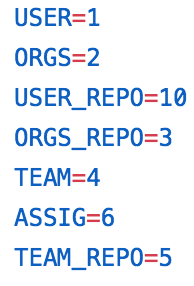
\includegraphics[height=2.5cm, width=2cm]{img/constantes.png}
    \column{0.6\linewidth}
    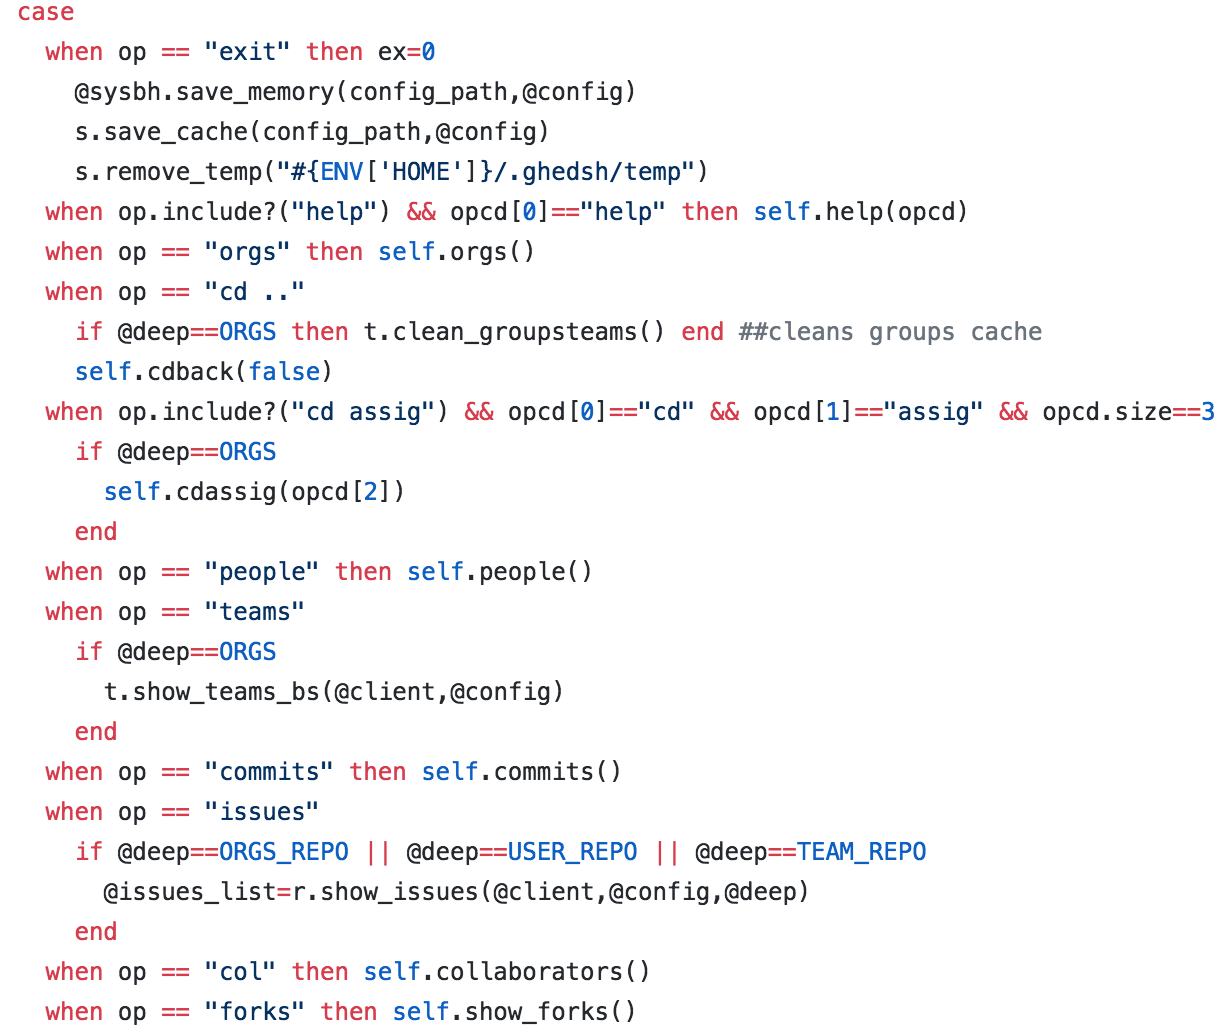
\includegraphics[height=7cm, width=7cm]{img/switch-smell.png}
  \end{columns}

\end{frame}

\begin{frame}
  \frametitle{Primera fase. Análisis}
  \framesubtitle{Long Method}
  {\it Long Method} se clasifica a nivel de método. Como su propio nombre indica,
  consiste en un método que ha crecido demasiado y dificulta saber qué es lo que realmente hace.
\end{frame}

\begin{frame}
  \frametitle{Primera fase. Análisis}
  \framesubtitle{Large Class}
    Large Class se clasifica dentro de los smells a nivel de clases. Indica que una clase ha crecido excesivamente en tamaño
    (God Object). Su funcionalidad puede descomponerse en clases más pequeñas.
\end{frame}


  %+++++++++++++++++++++++++++++++++++++++++++++++++++++++++++++++++++++++++++++++++++++++++++++++++++++++++
\subsection{Segunda fase. Refactorización}
\begin{frame}
\frametitle{Segunda fase. Refactorización}
  Esta fase se centra en eliminar las debilidades anteriormente comentadas. Gran parte de este proceso
  consistió en eliminar el {\it Switch Smell}, ya que era el más repetido a lo largo del código fuente.

\end{frame}

%+++++++++++++++++++++++++++++++++++++++++++++++++++++++++++++++++++++++++++++++++++++++++++++++++++++++++++
\begin{frame}
  \frametitle{Segunda fase. Refactorización}
  \framesubtitle{Strategy Pattern}
  Para eliminar el {\it Switch Smell} hemos aplicado el Patrón Estrategia ({\it Strategy Pattern}).
  \bigskip

  El propósito de este patrón es proporcionar una manera clara de definir familias de algoritmos y poder intercambiarlos fácilmente.
  
\end{frame}

\begin{frame}
  \frametitle{Segunda fase. Refactorización}
  \framesubtitle{Strategy Pattern}

  \centering
  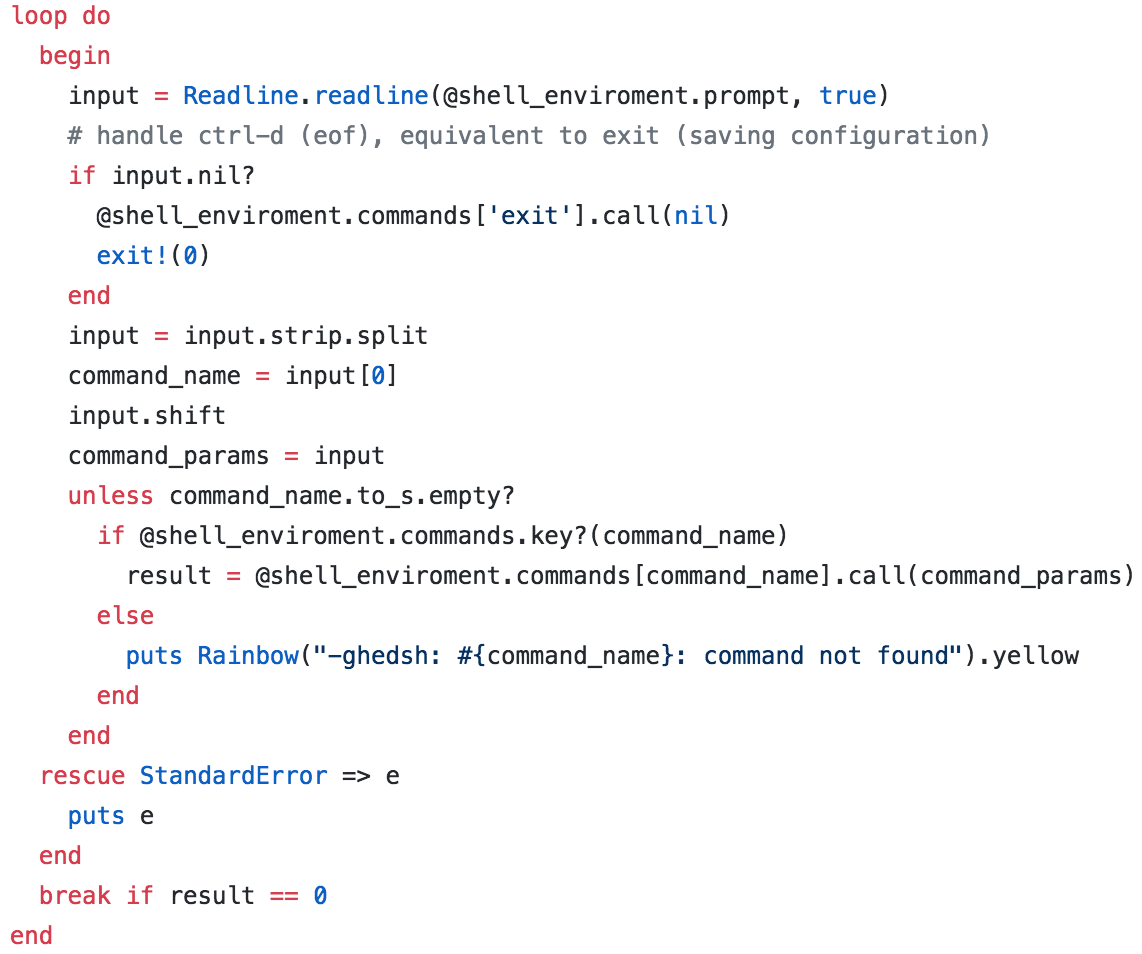
\includegraphics[height=7cm, width=7cm]{img/new-loop.png}
\end{frame}

\begin{frame}
  \frametitle{Segunda fase. Refactorización}
  \framesubtitle{Extract Method}

  \centering
  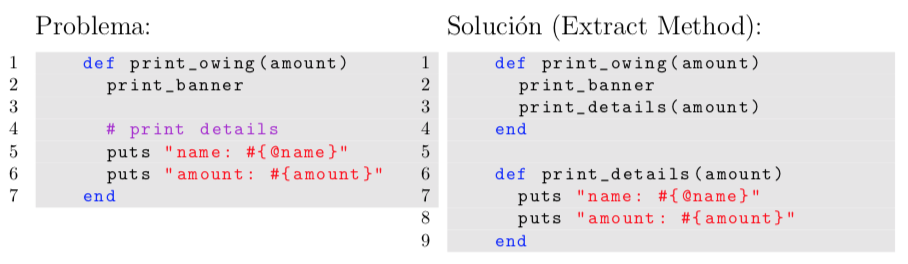
\includegraphics[height=3cm, width=10cm]{img/extract-method-example.png}
\end{frame}

\begin{frame}
  \frametitle{Segunda fase. Refactorización}
  \framesubtitle{Extract Class}

  Una clase debería tener una única responsabilidad.
  \bigskip

  \begin{itemize}
    \item Paso 1. Determinar qué se va a extraer.
    \item Paso 2. Crear una nueva clase.
    \item Paso 3. Renombrar la clase antigua.
  \end{itemize}
\end{frame}

%+++++++++++++++++++++++++++++++++++++++++++++++++++++++++++++++++++++++++++++++++++++++++++++++++++++++++++
\section{Resultados obtenidos}
\begin{frame}
\frametitle{Resultados obtenidos}
  Tras la etapa de desarrollo, {\it GitHub Education Shell} incorpora las siguientes características:
  \begin{itemize}
    \item Autenticación con credenciales de GitHub (OAuth).
    \item Conjunto de comandos
    \begin{itemize}
      \item Comandos del núcleo de {\it ghedsh}.
      \item Comandos incorporados ({\it built-in commands}).
      \item Comandos que dan soporte al proceso de evaluación.
    \end{itemize}
  \end{itemize}
\end{frame}

\begin{frame}
  \frametitle{Resultados obtenidos}
  \framesubtitle{Comandos del núcleo de {\it ghedsh}}

  \begin{itemize}
    \item \textbf{cd}: permite movernos entre repositorios, organizaciones, equipos, etc.
    \item \textbf{! ó bash}: interpreta la entrada del usuario como un comando tipo Unix.
  \end{itemize}

\end{frame}

\begin{frame}
  \frametitle{Resultados obtenidos}
  \framesubtitle{Comandos incorporados}

  \begin{minipage}[t]{0.48\linewidth}
    \centering
    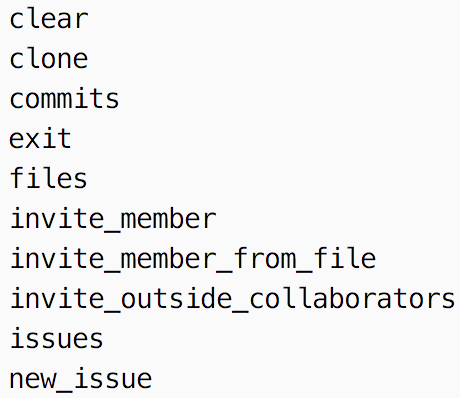
\includegraphics[height=4cm, width=4cm]{img/commands2.png}
  \end{minipage}%
  \begin{minipage}[t]{0.48\linewidth}
    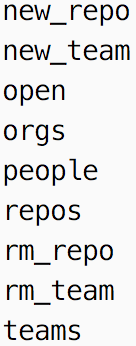
\includegraphics[height=4cm, width=1.5cm]{img/commands1.png}
  \end{minipage}

\end{frame}

\begin{frame}
  \frametitle{Resultados obtenidos}
  \framesubtitle{Comandos que dan soporte al proceso de evaluación}

  Tenemos los siguientes:
    \begin{itemize}
      \item \textbf{new\_eval}
      \item \textbf{foreach}
      \item \textbf{foreach\_try}
    \end{itemize}
\end{frame}

\begin{frame}
  \frametitle{Resultados obtenidos}
  \framesubtitle{new\_eval}
  \textbf{new\_eval}
  \bigskip

  Permite crear un repositorio de evaluación. Consiste en hacer uso de los submódulos de {\it git},
  de manera que se crea un ``súper repositorio'' que contiene como submódulos los proyectos que se van a evaluar.
  \bigskip

  \centering
  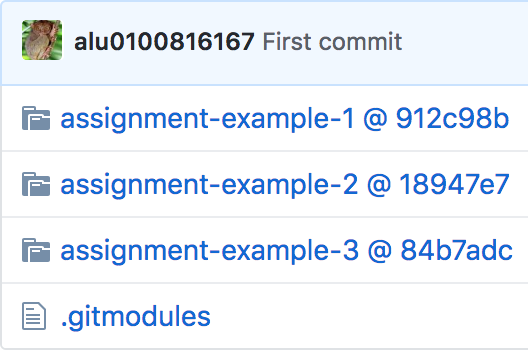
\includegraphics[height=3cm, width=4.5cm]{img/eval-preview.png}

\end{frame}

\begin{frame}[fragile]
  \frametitle{Resultados obtenidos}
  \framesubtitle{foreach y foreach\_try}
  \textbf{foreach}
  \bigskip

  Ejecuta para cada submódulo el comando especificado (por ejemplo, \verb git  \verb pull ). Internamente realiza \verb git  \verb submodule  \verb foreach .
  Si ocurre algún error en un submódulo durante la ejecución del comando, pasa al siguiente submódulo.
  \bigskip

  \textbf{foreach\_try}
  \bigskip

  Realiza lo mismo que \verb foreach . Sin embargo, \verb foreach_try  dentendrá su ejecución si ocurre
  algún error en un submódulo.

\end{frame}

\begin{frame}[fragile]
  \frametitle{Resultados obtenidos}
  \framesubtitle{foreach y foreach\_try}
  
  Hagámonos una pregunta:
  \bigskip

  \textbf{¿Y si en lugar de ejecutar un comando simple, hacemos uso de una librería o paquete que realiza tareas más complejas?}

\end{frame}

\begin{frame}[fragile]
  \frametitle{Resultados obtenidos}
  \framesubtitle{ghedsh-grade-node}
  
  Explico el paquete de ejemplo [....]

  \centering
  
\includegraphics[height=2.5cm, width=2.5cm]{img/ghedsh-grade-node.png}

\end{frame}
%+++++++++++++++++++++++++++++++++++++++++++++++++++++++++++++++++++++++++++++++++++++++++++++++++++++++++++
  
\section{Caso de uso}

\begin{frame}[allowframebreaks]
\frametitle{Caso de uso}

\end{frame}

%+++++++++++++++++++++++++++++++++++++++++++++++++++++++++++++++++++++++++++++++++++++++++++++++++++++++++++

\section{Conclusions and future work lines}
\begin{frame}[allowframebreaks]
  \frametitle{Conclusions and future work lines}

\end{frame}

%++++++++++++++++++++++++++++++++++++++++++++++++++++++++++++++++++++++++++++++ 

\section{Bibliografía}
\begin{frame}[allowframebreaks]
  \frametitle{Bibliografía}
  \bibliographystyle{ieeetr}
  \bibliography{presentacion_tfg}
  \nocite{*}
\end{frame}

\begin{frame}
  \frametitle{Fin de la presentación}
  \begin{center}
    \Huge{Gracias por su atención}
  \end{center}
\end{frame}

\end{document}
